\subsection{Motor}
\begin{tcolorbox}[colback=blue!5!white,colframe=blue!75!black,title=Motor eléctrico]
	Los motores eléctricos son máquinas que transforman la energía eléctrica en movimiento (energía cinética). Estos aparatos se componen, básicamente, del rotor y de un estator donde tiene bobinas inductoras desfasadas entre sí 120°
\end{tcolorbox}

\subsubsection{Especificaciones}
El motor (Figura \ref{fig:motor}) asincrónico que se utiliza es de la marca \textbf{Altium} perteneciente a la firma \textbf{Schneider Electric}. Las especificaciones se muestran a continuación \\
\paragraph*{Altium Eff2}

\begin{minipage}[t]{.5\textwidth}
	\begin{itemize}
		\item Tipo: TE2A90SP2
		\item Tensión nominal: 380 V
		\item Corriente nominal: 3.46 A
		\item Frecuencia nominal:  50 Hz.
		\item Potencia: 1.5kW / 2 HP
		\item Fases: 3
		\item Factor de Potencia: 0.84
	\end{itemize}
\end{minipage}
\begin{minipage}[t]{.5\textwidth}
	\centering\raisebox{\dimexpr \topskip-\height}{%
		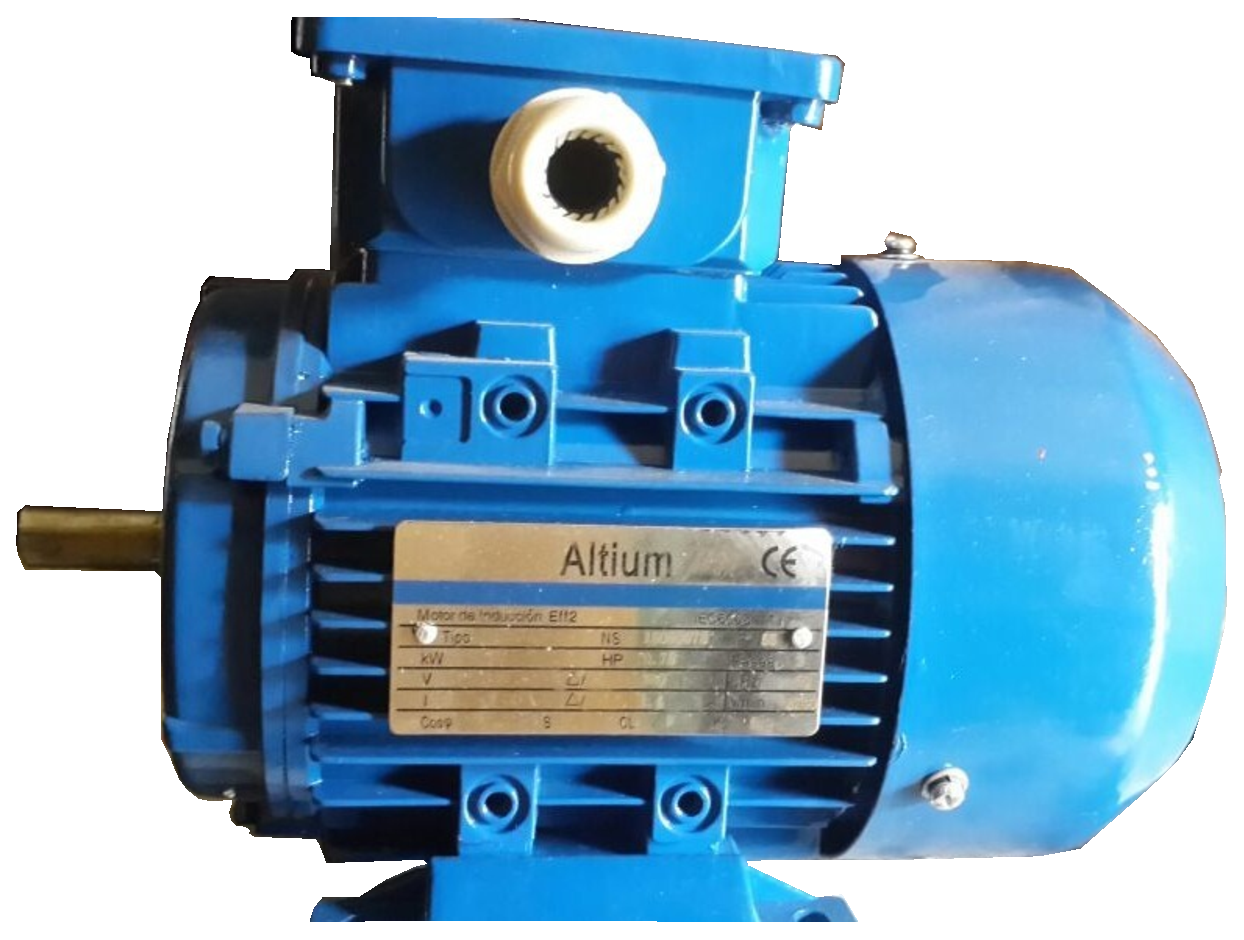
\includegraphics[scale=0.3]{motor.eps}}
	\captionof{figure}{Motor Altium}
	\label{fig:motor}

\end{minipage}

\subsection{Variador de velocidad}
\begin{tcolorbox}[colback=blue!5!white,colframe=blue!75!black,title=Variador de velocidad]
	Es utilizado para controlar la velocidad de giro de un motor.
	Para regular las revoluciones, se debe tener en cuenta las características del motor, ya que este tiene una curva propia de funcionamiento. Un variador es capaz de generar elementos control de aceleración, frenado, seguridad, control del torque y operaciones que mejoran la eficiencia energética.
\end{tcolorbox}

\subsubsection{Especificaciones}
El variador de velocidad que se utilizó pertenece a la marca \textbf{Schneider Electric} (Figura \ref{fig:variador}) y posee las siguientes características.
\paragraph*{Altivar 312}
\begin{minipage}[t]{.5\textwidth}
	\begin{itemize}
		\item 	Modelo: ATV312HU15N4
		\item   Tensión: 380-500 V
		\item 	Frecuencia: 50/60 Hz
		\item 	Potencia: 1.5kW / 2 HP
		\item 	Fases: 3
	\end{itemize}
\end{minipage}
\begin{minipage}[t]{.5\textwidth}
	\centering\raisebox{\dimexpr \topskip-\height}{%
		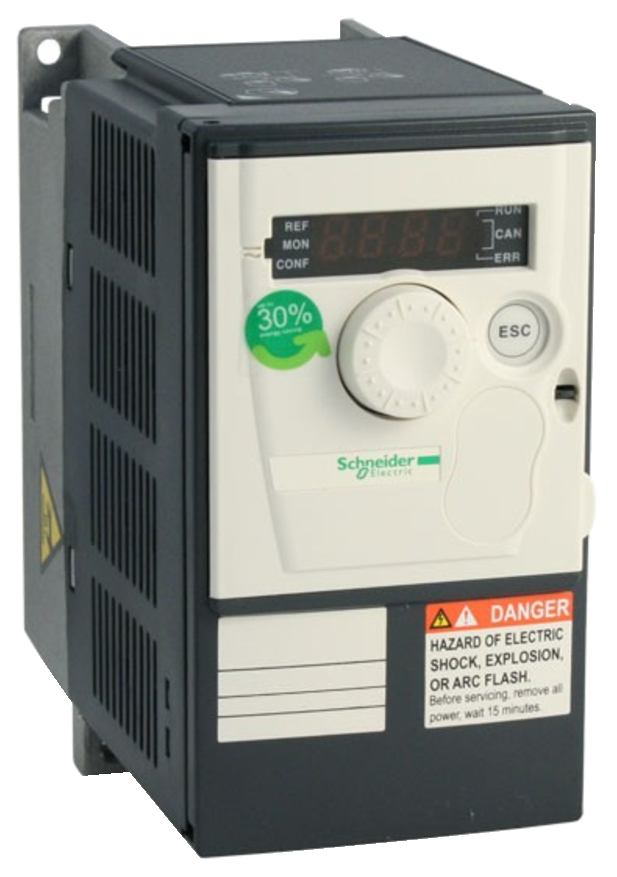
\includegraphics[scale=0.25]{variador.eps}}
	\captionof{figure}{Variador Altivar 312}
	\label{fig:variador}
\end{minipage}


Cabe destacar que el variador estima la velocidad de acuerdo a los parámetros del motor, por lo que para medir la velocidad verdadera se utiliza un tacómetro perteneciente al laboratorio.


\subsection{PLC}
\begin{tcolorbox}[colback=blue!5!white,colframe=blue!75!black,title=PLC]
	Es una computadora que se utiliza en la ingeniería de automatización para controlar procesos las industrias.
\end{tcolorbox}

\subsubsection{Módulos PLC M340}
El laboratorio cuenta con un PLC modular didáctico \ref{fig:didac} de la marca \textbf{Schneider Electric} de la familia \textbf{Modicon} modelo \textbf{M340} que posee los siguientes módulos:
\begin{itemize}
	\item BMX XBP 0400: bastidor para 4 módulos más la fuente de alimentación.
	\item BMX P34 2030: CPU 340-20 Ethernet CANopen.   (Comunicación)
	\item BMX ART 0414: 4 entradas TC/RTD con separación de potencial.
	\item BMX DDM 16022: 8 entradas digitales, y 8 salidas digitales por transistor PNP, todas ellas aisladas.
	\item BMX CPS 2000: Fuente de alimentación de 220V
\end{itemize}
\begin{center}
	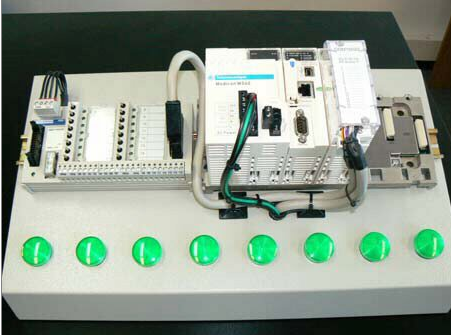
\includegraphics[scale=0.8]{educativo.png}
	\captionof{figure}{Módulo Didáctico PLC M340}
	\label{fig:didac}
\end{center}




